\documentclass[chicago]{emulateapj}
\usepackage{graphicx,amsmath,natbib,bm}
\usepackage[none]{hyphenat}
\usepackage{amsfonts}
\usepackage[top=1.3in, bottom=-0.3in, left=0.9in, right=0.35in]{geometry}
\usepackage{times}
\linespread{1.01}
\usepackage{enumitem}
\usepackage{framed}

\shortauthors{Y. Hezaveh}
\begin{document}

\title{Probing the inner kpc of massive lens galaxies with ALMA: Can the central images of strong lenses be detected?}
\author{Yashar D. Hezaveh, Philip J. Marshall, Roger D. Blandford}  
\affil{Kavli Institute for Particle Astrophysics and Cosmology, Stanford University, Stanford, CA, USA}

\begin{abstract}  
\noindent
We examine the prospects of detecting demagnified images of gravitational lenses in observations of strongly lensed mm-wave molecular emission lines with ALMA. We model the lensing galaxies as a superposition of a dark matter component, a stellar population, and a central supermassive black hole and forecast the detection of the central images for a range of relevant parameters (e.g. stellar core and black hole mass).
We find that over a large range of acceptable parameters, future deep observations of lensed molecular lines with ALMA will be able to detect the central images at $\gtrsim 3\sigma$ significance. We use Fisher analysis to examine the  constraints that could be placed on these parameters in various scenarios. 

\end{abstract}

%in Ferarrese 2006, $r_b$ varies from ~50 to 500 pc. 


\keywords{ black hole physics ---
gravitational lensing: strong ---
galaxies: formation ---
galaxies: high-redshift}



\section{introduction}
\begin{framed}
Probing the inner 0.5 kpc is interesting because: \\ \\1) SMBHs are there \\2) Various DM models have different predictions \\3) The stellar population profile is contains information about past mergers and BH-stellar population interactions. 
\\
\\
Mapping the matter density and decomposing these different components can thus shed light on various astrophysical phenomena.
%probing the inner 0.5 kpc of galaxies is interesting. 1) they contain SMBHs and the relationship of the SMBH mass to galaxies is intriguing and interesting. Dark matter models also have different and interesting predictions for the density of the central regions of galaxies (e.g. cored DM, or SIDM predictions). In addition, the history of galaxy mergers and black hole-stellar population interactions can be encoded in the stellar light profiles, resulting in different stellar  
\end{framed}

\begin{framed}
Stellar light profiles:
\\ \\
1) Massive galaxies often exhibit cored surface brightness profiles.  \\% (Cores sizes of order 50 -- 500 pc).
2) The most massive ellipticals are thought to form through gas-poor mergers.\\

3) The central structure of a merger without gas is dominated by the more concentrated of the two progenitors: the steeper central density cusp survives. \\

4) Since high-mass ellipticals are thought to be built from mergers of lower-mass ellipticals, which have steep central-density cusps, the cores in more massive ellipticals have to be the result of another (not merger) physical mechanism.  \\

5) The existence of cores thus, represents a challenge to our understanding of the merging process.\\


6) ``Black hole scouring''  has been suggested to produce a core.
\end{framed}

\begin{framed}
Explain ``Black hole scouring''.  \\
...\\
...\\
...\\
... whatever the mechanisms are, clear measurements of the central densities can be valuable to solve this puzzle and to shed light on the connection of SMBHs and galaxies. 
\end{framed}

\begin{framed}
Strong lensing: \\  \\
1) lensing is a well-known tool for mapping out mass \\ \\
2) strong lenses have been used to measure the einstein mass (e.g., X et al.), and the density skopes (Y et al.). \\ \\
3) Strong lensing formalism, predicts an odd number of images, with a central image that is \emph{demagnified} \\ \\
4) it has been known that the flux (i.e. demagnification) of the central image is very sensitive to the very inner regions of the density profiles: very peaky, singular density profiles, demagnify the image by very large amounts, whereas cored or shallow profile will result in bright central images. \\ \\

4) typically only an even number of images are observed,  suggesting that the central images are demagnified below the sensitivity of instruments. \\ \\

5) Additionally, another reason for lack of detection is that the central image is located at the center of the lensing galaxy, where i) the sensitivity is lower, due to photon noise of the lens ii) it is difficult to distinguish the flux of the central image from the emission from the lens. iii) if in optical, since they pass through the centers of galaxies there's a high chance of large absorption (in the lens)
\end{framed}


\begin{framed}
a review of central image observations, claims, and studies:\\ \\
Winn et al 2004 \\ Rusin et al 2005 \\Inada et al 2005, etc.
\end{framed}


\begin{framed}
Describe the newly discovered population of mm lenses + ALMA's observations: \\  \\
1) strong lenses in mm were discovered (SPT, Herschel, etc.) \\ \\
2) ALMA observations confirmed that they're all lensed and that the sources are at high z \\ \\
3) because they were selected by flux, + the high sensitivity of ALMA $->$ SNR is very high \\ \\
4) the sources have many molecular lines. If a central image of a \emph{molecular line} is observed it will be easily identifiable since it corresponds to the redshift of the source, and there will be no confusion that it may be associated with the lens. \\ \\
5) since these lines are in mm, there's very little (if any) absorption in the lens, so the flux doesn't decrease due to absorption
\end{framed}

\begin{framed}
motivation and description of the paper: \\ \\
1) Long ALMA observations of these molecular lines are likely to be carried out for various reasons (e.g. power spectrum of dark matter, measuring the mass of background black holes) .  \\ \\
2) In this paper we explore the possibility of detection of these central images in such deep observations, and investigate what we could learn about the innermost regions of galaxies from detection or non-detection of such central images.\\ \\
3) the paper is organized as: section 2 describes the simulations, section 3 presents the results and discuss them and conclude in section 5 \\ \\
4) we use $\Lambda$CDM cosmology of XXX
\end{framed}

\section{Simulations}
\begin{framed} description
We generate mock data cubes of gas emission in the source galaxy, lens the data cubes with a foreground halo, predict the ALMA visibilities, and use the visibilities to estimate the detection significance of the central image for various parameters. 
The gas in the source galaxy is modeled as a collection of 5 Gaussian clumps with FWHM of XX, distributed over XX kpc and each separated in a different channel.
and an intrinsic velocity dispersion  of 10 $km/s$ (FWHM) similar to observations of \citet{Davis:13}. 
The choice of two discrete rings is made to enforce resolving the inner 50 pc region for a black hole mass measurement. We point out, however, that assuming a more general case (e.g. an exponential disk) does not change the results \citep[see Figure 2 of ][]{Davis:2014}.
The velocity integrated flux of the circumnuclear ring is set to 4 $mJy\, km/s$. 
This value is calculated by scaling the flux of the circumnuclear CO gas in Arp 220 to to z=2 \citep{Sakamoto:99}.
The rings are concentric and in circular orbits. The rotational velocity of each point in the rings is calculated based on the enclosed mass contributed from the galaxy mass model and the mass of the central black hole. The black hole is given a mass of $M_{\mathrm{BH}}=5\times 10^{8} M_{\odot}$.
We model the galaxy density with an isothermal profile ($\rho\propto r^{-2}$) with a central velocity dispersion of 200 km/s. 
The line-of-sight velocities are calculated to generate a frequency-position data cube. Figure \ref{f:f1} shows a velocity-position diagram extracted from the data cube. The data comprises 100 frequency channels covering 800 km/s. 


Each layer of the data cube is lensed with the foreground halo to  generate a lensed cube. We use a Singular Isothermal Ellipsoid (SIE) mass model for the lens galaxy \citep[$\rho\propto r^{-2}$,][]{Kormann:94}, placed at $z_l=0.5$ and place the source at $z_s=2.0$. The central velocity dispersion of the lens is set to 180 $km/s$, which is typical for galaxy-galaxy lensing systems \citep[e.g.][]{hezaveh:13b}. 


To predict the visibilities we calculate the ALMA $uv$-coverage for a 5-$hr$ long observation with the most extended antenna configuration (full array), using the $simobserve$ task of Common Astronomy Software Applications package, which results in an angular resolution of $\sim20\, \, milli$-$arcsec$ at an observing frequency of 240 GHz. 
The visibilities for each channel are calculated by computing the 2D Fourier transform of the corresponding layer of the data cube and resampling the Fourier transform maps over the uv-coverage. 
The noise is estimated using ALMA sensitivity calculator for a channel width of 8 km/s at 240 GHz. 
We use finite differencing of visibilities to calculate the Fisher information and the parameter covariance matrix to calculate the significance of black hole mass measurement.

When the background source only consists of the two rings described above, the lens model parameters have large uncertainties and are mildly degenerate with the mass of the black hole. 
A realistic source galaxy, however, will consists of many other components, extended over kilo-parsec scales, which if included in lens models, can strongly constrain the lens parameters.
We run five simulations in which the background source is embedded in an extended Gaussian clump with a radius of 1 kpc and a flux of 1 Jy km/s \citep[typical for SMGs, see][]{Bothwell:12}. We find that in these simulations, the lens parameters are extremely constrained and the effect of marginalization over them barely reduces the significance of black hole mass measurements ($\lesssim 0.05\, \sigma$). This suggests that when the full structure of the source galaxies are included in models, the lens parameters do not significantly contribute to the black hole mass uncertainties. Therefore, to reduce the computational cost of simulations, we do not marginalize over the lens parameters.
%\\ \\ \\ \\ \\ \\ \\ \\ \\ \\ \\ \\ \\ \\ \\ \\ \\ \\ \\ \\ \\ \\ \\ \\ \\ \\ \\ \\ \\ \\ \\ \\ \\ \\ \\ \\ \\ \\ \\ \\ \\ \\ \\ \\ \\ \\ \\ \\ \\ \\ \\ \\ \\ \\ \\ \\ \\ \\ \\ \\ \\ \\ \\ \\ \\ \\ \\ \\ \\ \\ \\ \\ \\ \\ \\ \\ \\ \\ \\ \\ \\ 
\end{framed}


\section{Results and Discussions}
%\begin{framed}
%\end{framed}

%\begin{framed}
%\end{framed}

%\begin{framed}
%\end{framed}

%\begin{framed}
%\end{framed}




\newpage

\begin{figure}
\begin{center}
\centering
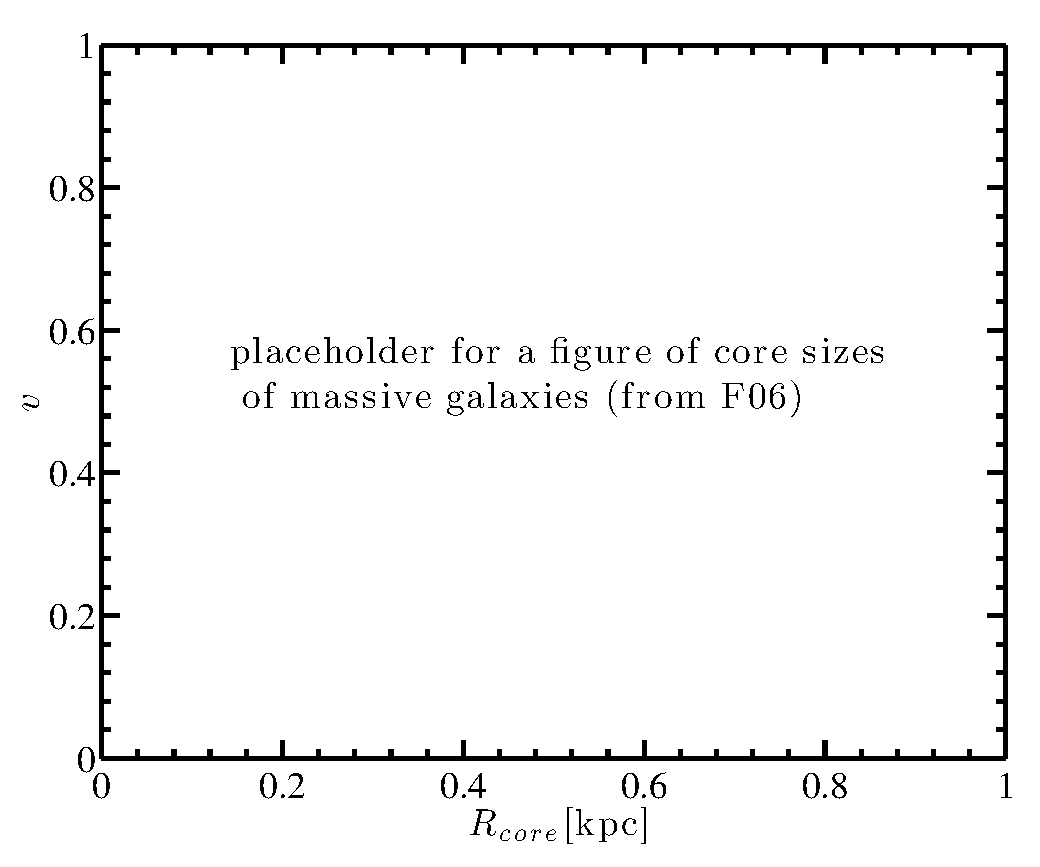
\includegraphics[trim= 0 0 5 6, clip, width=0.45\textwidth]{figures/f_01.eps}
\centering
\end{center}
\caption{ illustration of the central image in 2 cases: 
\label{f:f2}}
\end{figure}


\begin{figure}
\begin{center}
\centering
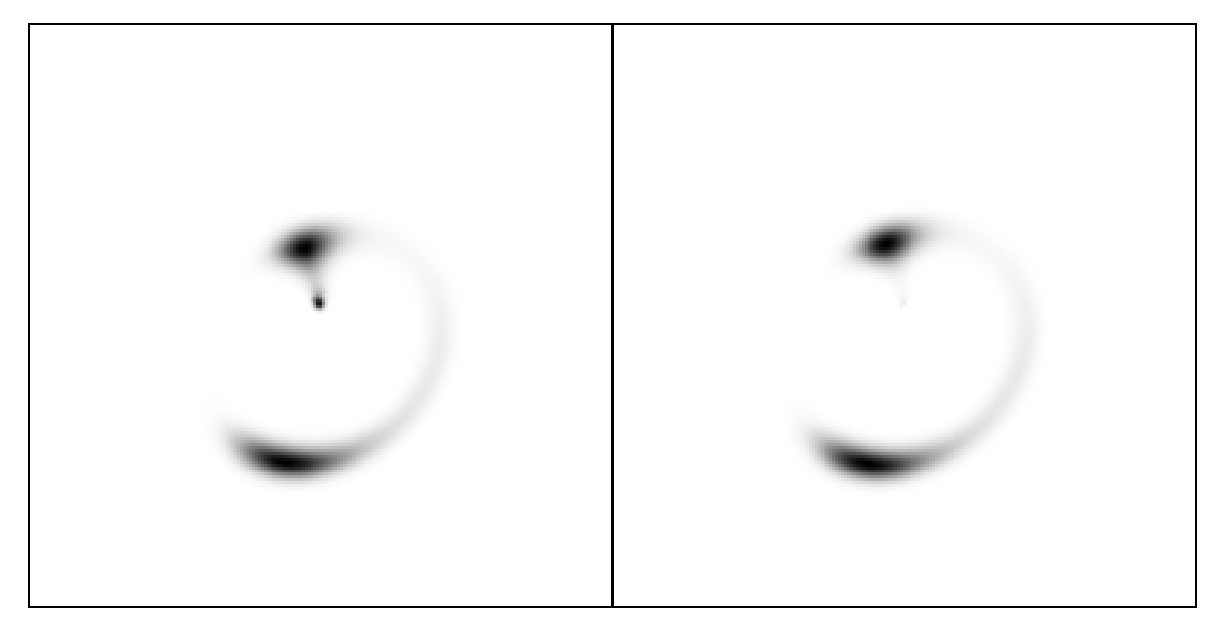
\includegraphics[trim= 0 0 0 0, width=0.45\textwidth]{figures/f_02.eps}
\centering
\end{center}
\caption{ illustration of the central image in 2 cases: 
\label{f:f2}}
\end{figure}


\begin{figure}
\begin{center}
\centering
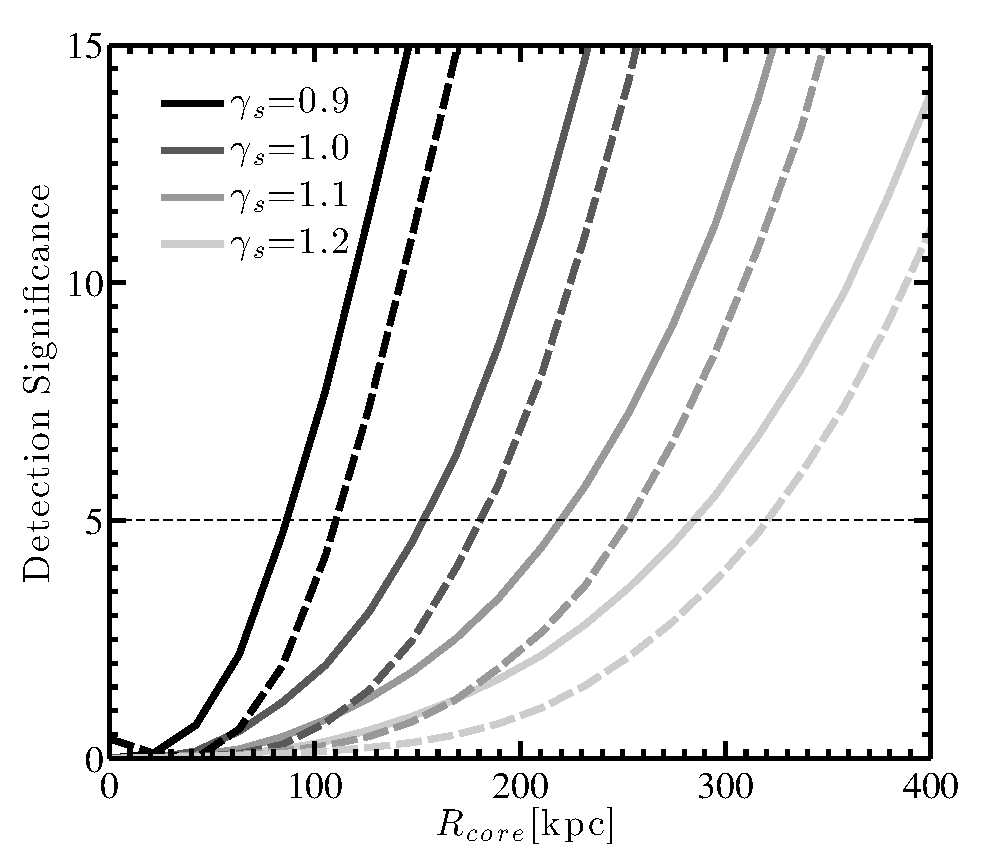
\includegraphics[trim= 0 0 0 0, width=0.45\textwidth]{figures/f_03.eps}
\centering
\end{center}
\caption{ Significance of detection of the central image as a function of the stellar core size. The colors correspond to different slopes of the stellar component. The solid curves correspond to a case without a SMBH while the dashed line show the result of a simulation which includes a $2\times10^8M_{\odot}$ SMBH at its center.
\label{f:f2}}
\end{figure}


\begin{figure}
\begin{center}
\centering
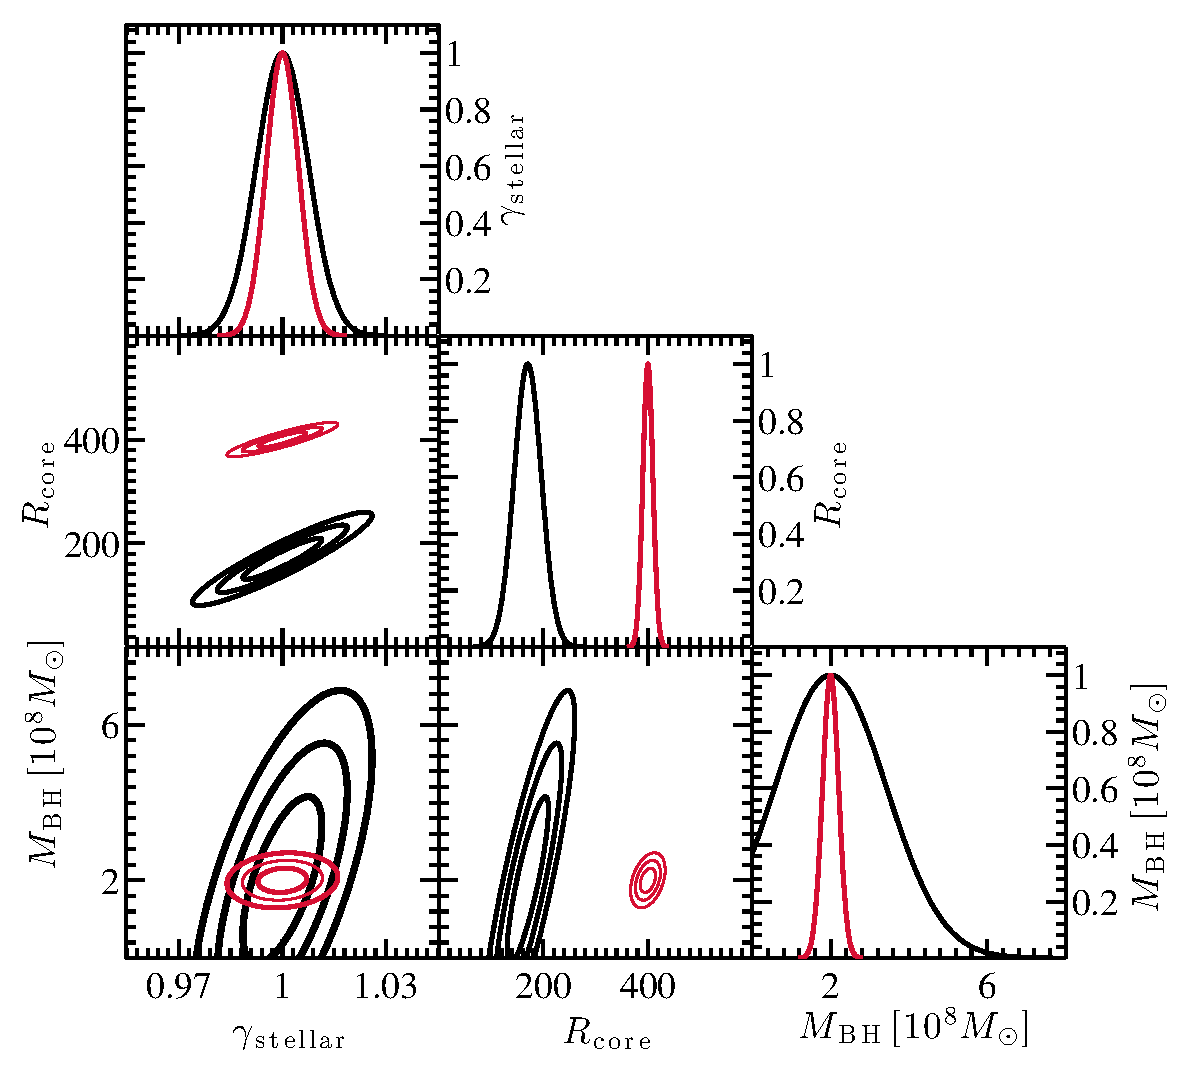
\includegraphics[trim= 0 0 0 0, width=0.45\textwidth]{figures/f_04.eps}
\centering
\end{center}
\caption{ Covariance matrix of parameters for a few different scenarios.
\label{f:f2}}
\end{figure}



\section{Conclusion}

\acknowledgements{
}





\end{document}
